\lstset{language=Java, numbers=left, numberstyle=\tiny, stepnumber=2, numbersep=5pt}
\chapter{Introduction}
\label{intro}
As the last few years and decades have seen ever-increasing amounts of data analyzed and managed in ever shorter periods of time, a challenge faced by the IT industry has been the limited computing power of individual machines and simple networks. Tasks are constantly evolving, so they need more and more computing power to solve them.\\
In order to solve these problems, various techniques have been developed that help to continuously improve the performance of the machines. These include supercomputers, computer clusters, and various methods and algorithms that can be summarized under the term High Performance Computing.\\
This workshop introduces the programming model \textbf{MapReduce} and a simulation of the model based on the \textbf{Hadoop} framework. The aim of this workshop was to use the Hadoop Simulation HSim to gain a basic understanding of the functionality of MapReduce.
%%%%%%%%%%%%%%%%%%%%%%%%%%%%%%%%%%%%%%%%%%%%%%%%%%%%%%%%%%%%%%%%%%%%%%%%%%%%%%%%%%%%%%%%%%%%%%%%%%%%%%%%%
%%%%%%%%%%%%%%%%%%%%%%%%%%%%%%%%%%%%%%%%%%%%%%%%%%%%%%%%%%%%%%%%%%%%%%%%%%%%%%%%%%%%%%%%%%%%%%%%%%%%%%%%%
%%%%%%%%%%%%%%%%%%%%%%%%%%%%%%%%%%%%%%%%%%%%%%%%%%%%%%%%%%%%%%%%%%%%%%%%%%%%%%%%%%%%%%%%%%%%%%%%%%%%%%%%%
\chapter{High Performance Computing With MapReduce and Hadoop}
\label{high}
As already mentioned in the introduction, MapReduce was introduced as a programming model to process large amounts of data (Big Data) in parallel on several machines. This reduces processing time, since the load can be distributed over multiple machines.\\
The following chapters briefly explain the basics of this workshop. First, MapReduce and its functionality are described. This is followed by a short introduction to Hadoop.
\section{MapReduce}
\label{mapreduce}
Mapreduce is a programming model that addresses the processing and analysis of large amounts of data using a distributed, parallelized approach \cite[][]{DG04}. The data to be processed is divided into several data blocks of the same size. These data blocks are processed in parallel and independently of each other. These different blocks are the inputs for a \textbf{mapping} function that performs filtering and sorting \cite[][]{BI01}. Each block receives a unique key. The resulting key value pairs now enter a process called \textbf{"shuffling"}. Therefore, the key value pairs are assigned to the correct nodes that are defined by the key. In other words, the shuffling process sorts the data from the separate mapping blocks into new blocks according to the key. Each block contains pairs with the same key but different values. These are required for the next to last step of the MapReduce process: \textbf{reducing}. The reduction phase cannot begin until the mapping phase is complete. In this phase, each value of a block is combined to its key so that you get a new key value pair, where the new value is a list of the old values. The last step is to combine all the pairs in a data block. This is the final result of the MapReduce process \cite[][]{TW15}. Large amounts of data are thus divided into much smaller blocks, which are processed in parallel and independently from each other and finally reassembled. MapReduce simplifies and accelerates parallel processing and analysis of large amounts of data and is therefore very popular in the big data area. Figure \ref{mapreducepic} shows an example with all required steps for the MapReduce programming model with simple datasets
\\
There are several implementations of the MapReduce programming model. One of these is described in the next chapter.
\begin{figure}[H]
	\centering
	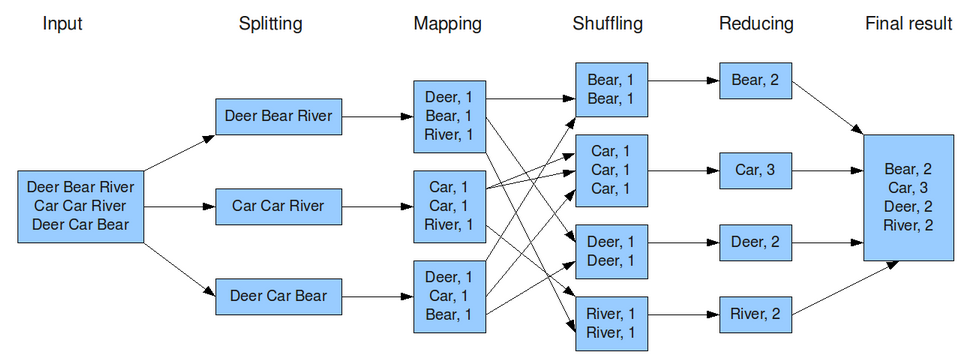
\includegraphics[width=1.0\linewidth]{mapreduce.PNG}
	\caption[Caption for LOF]{The MapReduce model\footnotemark}
	\label{mapreducepic}
\end{figure}
\footnotetext{image-source: https://cs.calvin.edu/courses/cs/374/exercises/12/lab}

\section{Hadoop}
\label{hadoop}
Apache Hadoop is a framework that allows distributed processing of large amounts of data across clusters of computers with simple programming models. It supports scalability from individual servers to thousands of computers, each with local calculations and storage \cite[][]{AP02}. Hadoop is based on Java and consists of four main components:
\begin{itemize}
	\item Hadoop Common
	\item Hadoop Distributed File System (HDFS)
	\item Google's MapReduce-algorithm
	\item Yet Another Resource Negotiator (YARN)
\end{itemize}
Hadoop Common provides the basic functions and tools for the other modules of the software. The HDFS will be described in the next sub-section. The MapReduce-algorithm is based on the MapReduce programming Model (s. Chapter \ref{mapreduce}) and offers the same functionality. The Yet Another Resource Negotiator (YARN) can manage the resources in a computer cluster and dynamically allocate the resources of a cluster to different jobs. YARN uses queues to determine the capacities of the systems for the individual tasks \cite[][]{NL01}. 
\\
Hadoop uses a master-slave architecture to distribute the data to be processed on several machines inside a cluster. A client transfers a job to the master node that is connected to the slaves in the cluster. The JobTracker of the master node controls the MapReduce job and reports it to a TaskTracker of a slave node. Within a slave node there are one or more data nodes as well as one or more Mappers and Reducers, which execute the MapReduce algorithm. In the event of an error, the JobTracker of the master node will reschedule the task to the same or a different slave node, depending on what is most efficient. This makes Hadoop very fault-tolerant and ensures that the entire process does not have to be aborted and restarted in the event of an error. \cite[][]{RO01}
\\
However, this alone is not enough to prevent the process from being terminated. If a master-node fails, all MapReduce processes that are processed by its associated slaves are also affected. Therefore, the master defines checkpoints after completion of single processing steps. In the event of an error, another master node can then continue where the failed master stopped and the process does not have to be rolled back completely. Figure \ref{master-slave} shows the Hadoop's Master-Slave architecture:
\begin{figure}[H]
	\centering
	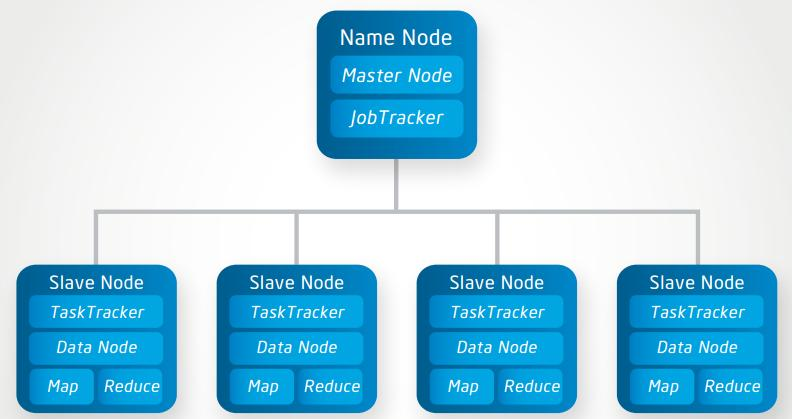
\includegraphics[width=1.0\linewidth]{master-slave.jpg}
	\caption[Caption for LOF]{The Hadoop Master-Slave Architecture\footnotemark}
	\label{master-slave}
\end{figure}
\footnotetext{image-source: http://www.rosebt.com/blog/hadooparchitecture-and-deployment}
\subsection{Hadoop Distributed File System (HDFS)}
The Hadoop Distributed File System (HDFS) is the primary data storage system used by Hadoop applications \cite[see][]{MR01}. It is a distributed file system that handles large data sets running on commodity hardware. HDFS splits the input data into data blocks and distributes them to independent nodes so that the data can be processed in parallel. For fault tolerance reasons, HDFS copies each piece of data several times and sends these copies to different racks (\textbf{replication}). This ensures the accessibility to the required data elsewhere in this cluster if a job node fails.\\
The structure consists of a name node and several data nodes according to the master-slave principle. The name node thus assumes the role of the master and is responsible for managing and coordinating the data in the clusters. The name-node contains metadata including the data replicas, checkpoints (s. Chapter \ref{hadoop}) and other important information, while the data nodes contain the actual data to be processed. Figure \ref{hdfs} shows the Hadoop Distributed File System Architecture and the ongoing read and write processes to the file system. 
\begin{figure}[H]
	\centering
	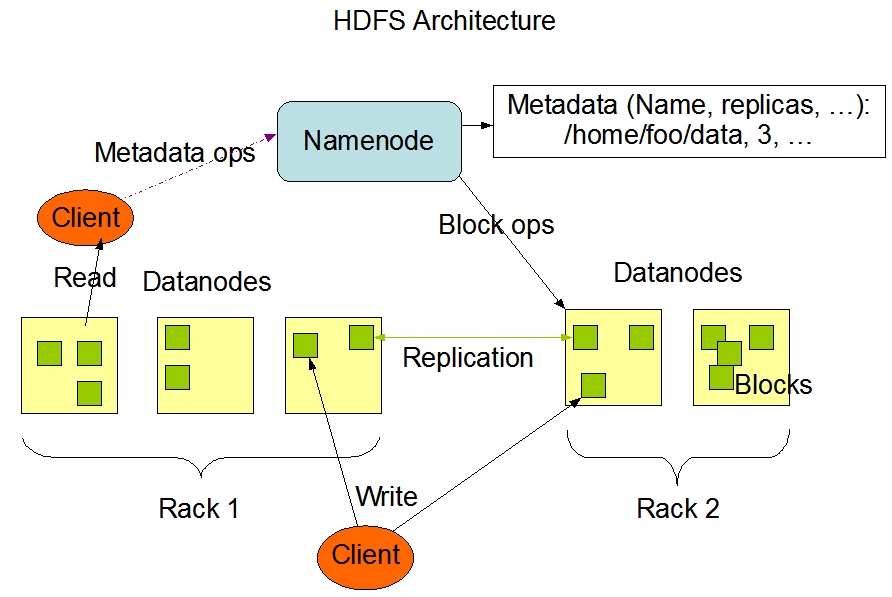
\includegraphics[width=1.0\linewidth]{hdfs.PNG}
	\caption[Caption for LOF]{The Hadoop Distributed File System Architecture\footnotemark}
	\label{hdfs}
\end{figure}
\footnotetext{image-source: https://hadoop.apache.org/docs/r1.2.1/hdfs\_design.html}
%%%%%%%%%%%%%%%%%%%%%%%%%%%%%%%%%%%%%%%%%%%%%%%%%%%%%%%%%%%%%%%%%%%%%%%%%%%%%%%%%%%%%%%%%%%%%%%%%%%%%%%%%
%%%%%%%%%%%%%%%%%%%%%%%%%%%%%%%%%%%%%%%%%%%%%%%%%%%%%%%%%%%%%%%%%%%%%%%%%%%%%%%%%%%%%%%%%%%%%%%%%%%%%%%%%
%%%%%%%%%%%%%%%%%%%%%%%%%%%%%%%%%%%%%%%%%%%%%%%%%%%%%%%%%%%%%%%%%%%%%%%%%%%%%%%%%%%%%%%%%%%%%%%%%%%%%%%%%
\chapter{Hadoop's Parameters}
\label{params}
Before starting the simulation of Hadoop in the next chapter, a closer look is taken at the parameters of Hadoop, which can be manipulated in the simulation to get different results. Table 3.1 shows an overview over the most important Hadoop parameter:
\begin{table}[H]
	\centering
	\label{parameters}
	\begin{tabular}{|l|l|}
		\hline
		\textbf{Configuration Parameters}             & \textbf{Default Values} \\ \hline
		io.sort.factor                                & 10                      \\ \hline
		io.sort.mb                                    & 100                     \\ \hline
		io.sort.spill.percent                         & 0.8                     \\ \hline
		mapred.reduce.tasks                           & 1                       \\ \hline
		mapreduce.tasktracker.map.tasks.maximum       & 2                       \\ \hline
		mapreduce.tasktracker.reduce.tasks.maximum    & 2                       \\ \hline
		mapred.child.java.opts                        & 200                     \\ \hline
		mapreduce.reduce.shuffle.input.buffer.percent & 0.7                     \\ \hline
		mapred.reduceparallel.copies                  & 5                       \\ \hline
		mapred.compress.map.output                    & False                   \\ \hline
		mapred.output.compress                        & False                   \\ \hline
	\end{tabular}
	\caption{Most important Hadoop parameters}
\end{table}

Each of these parameter can be changed to change the way Hadoop is working on large datasets. The following decriptions for each parameter are directly taken from Appache's offical documentation\footnote{https://hadoop.apache.org/docs/r1.0.4/mapred-default.html}:
\\\\
\textbf{io.sort.factor:} This is the number of streams Hadoop uses to sort the files in parallel. Keep note that this determines the number of open files that have to be handled.
\\\\
\textbf{io.sort.mb:} This is the total amount of buffer memory Hadoop sorts the files in MB. The default value per merge stream accounts for 1MB, which should minimize seeks.
io.sort.spill.percent: The soft limit in either the buffer or record collection buffers. Once reached, a thread will begin to spill the contents to disk in the background. Note that this does not imply any chunking of data to the spill. A value less than 0.5 is not recommended.
\\\\
\textbf{mapred.reduce.tasks:} The default number of reduce tasks per job. Typically set to 99\% of the cluster's reduce capacity, so that if a node fails the reduces can still be executed in a single wave. Ignored when mapred.job.tracker is "local".
\\\\
\textbf{mapreduce.tasktracker.map.tasks.maximum:} The maximum number of map tasks that will be run simultaneously by a task tracker.
\\\\
\textbf{mapreduce.tasktracker.reduce.tasks.maximum:} The maximum number of reduce tasks that will be run simultaneously by a task tracker.
\\\\
\textbf{mapred.child.java.opts:} Java opts for the task tracker child processes. The following symbol, if present, will be interpolated: @taskid@ is replaced by current TaskID. Any other occurrences of '@' will go unchanged. For example, to enable verbose gc logging to a file named for the taskid in /tmp and to set the heap maximum to be a gigabyte, pass a 'value' of: -Xmx1024m-verbose:gc -Xloggc:/tmp/@taskid@.gc The configuration variable mapred.child.ulimit can be used to control the maximum virtual memory of the child processes.
\\\\
\textbf{mapreduce.reduce.shuffle.input.buffer.percent:} The percentage of memory to be allocated from the maximum heap size to storing map outputs during the shuffle.
\\\\
\textbf{mapred.reduceparallel.copies:} The default number of parallel transfers run by reduce during the copy(shuffle) phase.
\\\\
\textbf{mapred.compress.map.output:} Should the outputs of the maps be compressed before being sent across the network. Uses SequenceFile compression.
\\\\
\textbf{mapred.output.compress:} Should the job outputs be compressed?

These are just a few selected parameters that can be changed to influence Hadoop's runtime behavior. The complete list can be found here: \cite[see][]{AP03}. Now that the theoretical basics have been sufficiently explained and the parameters for the simulation described, it is time to move on to the actual topic of this assignment. The next chapter will introduce HSim and show how to change the parameters listed above to achieve different results in the simulation.
%%%%%%%%%%%%%%%%%%%%%%%%%%%%%%%%%%%%%%%%%%%%%%%%%%%%%%%%%%%%%%%%%%%%%%%%%%%%%%%%%%%%%%%%%%%%%%%%%%%%%%%%%
%%%%%%%%%%%%%%%%%%%%%%%%%%%%%%%%%%%%%%%%%%%%%%%%%%%%%%%%%%%%%%%%%%%%%%%%%%%%%%%%%%%%%%%%%%%%%%%%%%%%%%%%%
%%%%%%%%%%%%%%%%%%%%%%%%%%%%%%%%%%%%%%%%%%%%%%%%%%%%%%%%%%%%%%%%%%%%%%%%%%%%%%%%%%%%%%%%%%%%%%%%%%%%%%%%%
\chapter{HSim}
\label{hsim}
As already mentioned in the introduction, no complete cluster is being set up for this workshop, as the effort would have been far too much. Instead the provided software \textit{HSim} was used, which provides a simulated Hadoop environment with several machines, routers and nodes. HSim is based on Java and Hadoop and it offers the possibility to adjust different Hadoop parameters and to display the effects on the simulation realistically. Figure \ref{hsim} shows HSim's main user interface while running a simulation.
\begin{figure}[H]
	\centering
	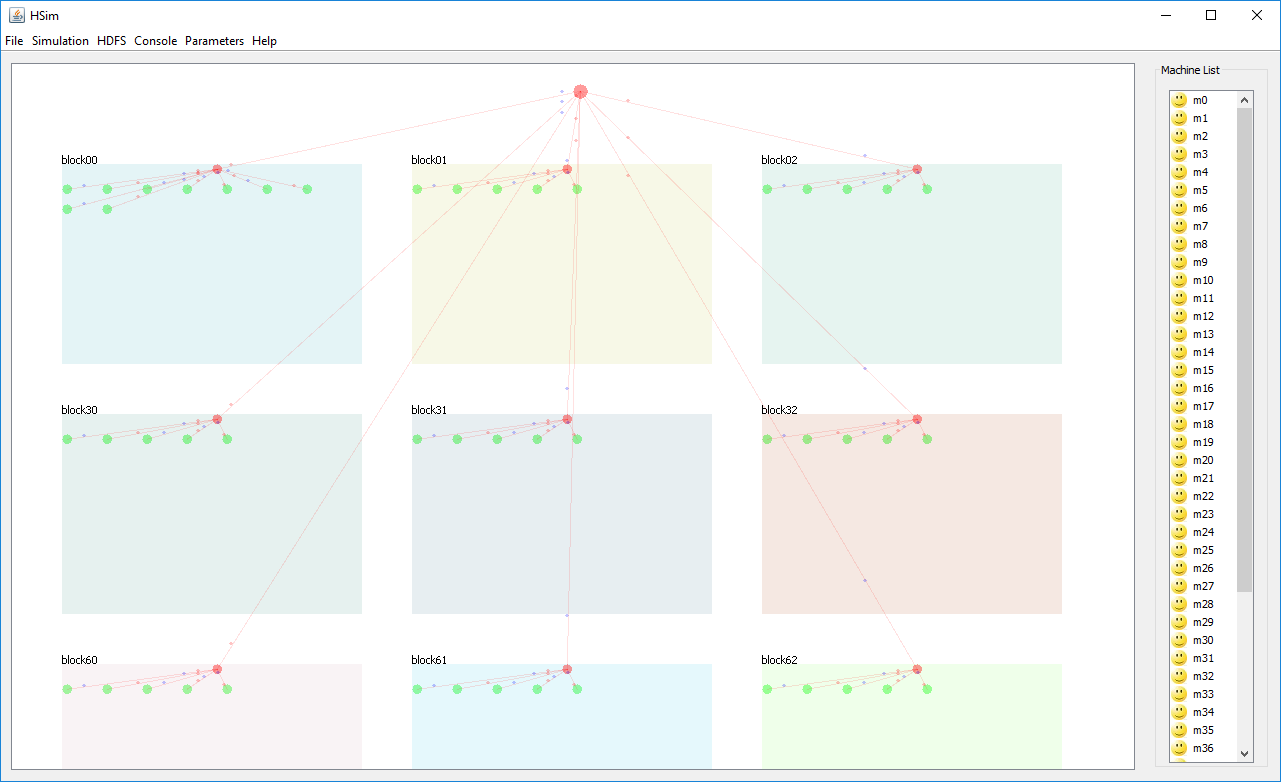
\includegraphics[width=1.0\linewidth]{hsim.png}
	\caption[Caption for LOF]{Screenshot of HSim's User Interface during a running Simulation}
	\label{hsim-pic}
\end{figure}
The rectangles in different colors represent the individual racks of the simulated Hadoop cluster. Each rack has multiple machines that are displayed as green dots. The red dots, of which each rack has one, are the routers. The red dot at the top edge is the master node, which splits the input data and distributes it to the routers of the racks. On the right hand side there is a list of all machines. The next figure \ref{machine-state} shows the machine state window that appears when double clicking on one of the machines.
\begin{figure}[H]
	\centering
	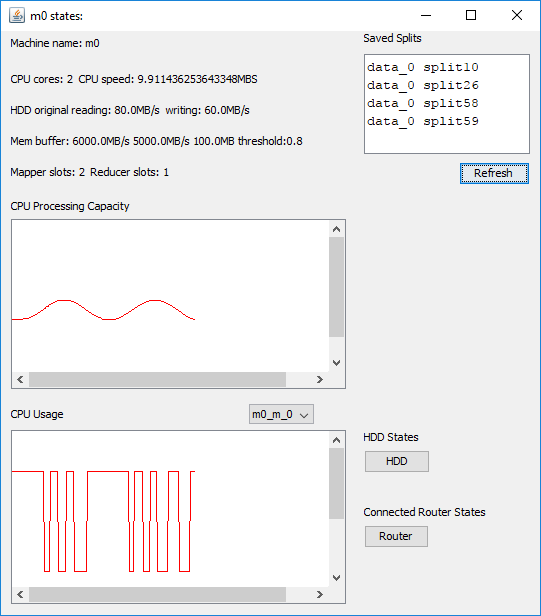
\includegraphics[width=0.75\linewidth]{machine-state.png}
	\caption[Caption for LOF]{Screenshot of the first machine's state window during a running Simulation}
	\label{machine-state}
\end{figure}
The performance of the individual machines can be observed here at the runtime of the simulation. The next figure \ref{hsim-console} shows the console that can be opened from HSim's main UI (see Figure \ref{hsim-pic}).
\begin{figure}[H]
	\centering
	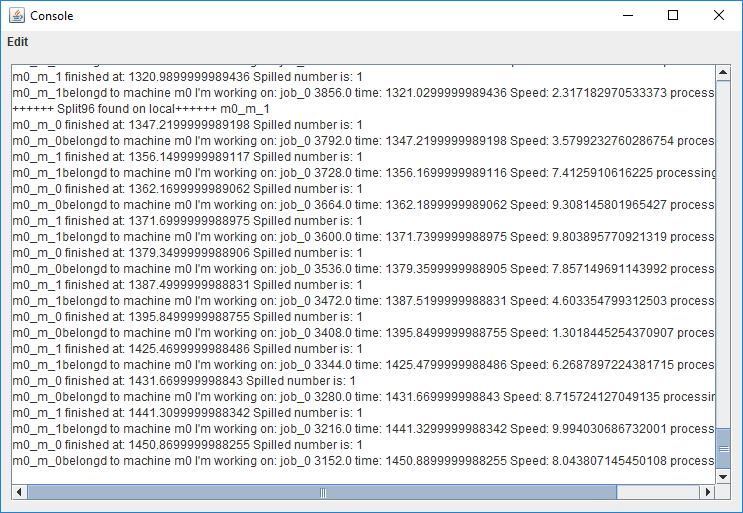
\includegraphics[width=0.85\linewidth]{hsim-console.png}
	\caption[Caption for LOF]{Screenshot of HSim's Console during a running Simulation}
	\label{hsim-console}
\end{figure}
From here, the individual processes for the individual jobs running on the various machines can be tracked at runtime. The runtimes required by the individual machines for a job are measured and displayed.
\\\\
The different Hadoop parameters (see chapter \ref{params}) can be set using a configuration file. For the following simulation, the presetting with a Hadoop cluster of 49 individual machines was used. In the next chapter, the influence of four different Hadoop parameters on the runtime of the simulation will be investigated.
%%%%%%%%%%%%%%%%%%%%%%%%%%%%%%%%%%%%%%%%%%%%%%%%%%%%%%%%%%%%%%%%%%%%%%%%%%%%%%%%%%%%%%%%%%%%%%%%%%%%%%%%%
%%%%%%%%%%%%%%%%%%%%%%%%%%%%%%%%%%%%%%%%%%%%%%%%%%%%%%%%%%%%%%%%%%%%%%%%%%%%%%%%%%%%%%%%%%%%%%%%%%%%%%%%%
%%%%%%%%%%%%%%%%%%%%%%%%%%%%%%%%%%%%%%%%%%%%%%%%%%%%%%%%%%%%%%%%%%%%%%%%%%%%%%%%%%%%%%%%%%%%%%%%%%%%%%%%%
\chapter{Evaluation}
\label{eval}
To get an impression of how changes to different parameters affect the runtime behavior of a real Hadoop cluster, the parameters' dataSize',' sortFactor' as well as' requiredMappers' and' requiredReducers' were assigned different values and then the simulation was started with these values. For each value change the simulation ran ten times and from each run the runtime was measured and afterwards an average value was calculated.
\\
Three different measurements have been made for the runtime. The \textbf{upload} time specifies the time that the Hadoop cluster would need under normal conditions to upload a job with the configured amount of data. The \textbf{mapping} time includes the time, which the simulated Hadoop cluster needs for the mapping step of the MapReduce algorithm and the already measured upload time. Finally, the \textbf{job} time indicates how long the simulated Hadoop cluster takes to process the configured job. This includes the mapping time as well as the time required by the cluster for the shuffling and reducing (see chapter \ref{mapreduce}).
\section{Changing the dataSize}
The first parameter that has been changed for the simulation is the amount of data for the job to be processed by the cluster. Figure \ref{datasize-table} shows a table with the individual amounts of data in megabytes as well as the respective average value for the different time measurements in seconds. 
\begin{figure}[H]
	\centering
	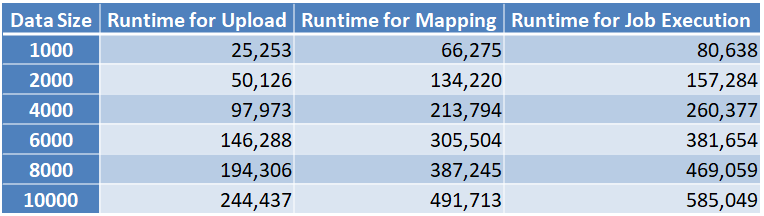
\includegraphics[width=1.0\linewidth]{datasize-table.PNG}
	\caption[Caption for LOF]{DataSize/RunTime table}
	\label{datasize-table}
\end{figure}
The graph in the figure \ref{datasize-chart} shows the dependency between the data size and the run time:
\begin{figure}[H]
	\centering
	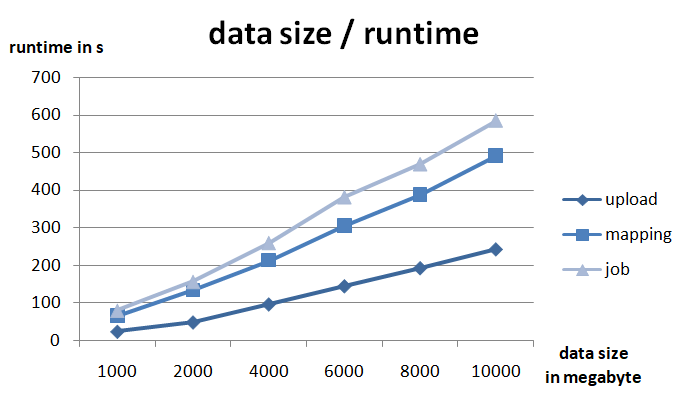
\includegraphics[width=0.85\linewidth]{datasize-chart.PNG}
	\caption[Caption for LOF]{DataSize/RunTime chart}
	\label{datasize-chart}
\end{figure}
It becomes clear that especially the time required by the cluster to upload the data increases almost linearly in relation to the data volume. Meanwhile, the amount of data seems to have less influence on the time required for mapping and reducing than I expected.
\section{Changing the sortFactor}
The next parameter that has been changed is the sort factor. Figure \ref{sortfactor-table} shows a table with different settings for the sort factor parameter and the resulting average values of the individual time measurements.
\begin{figure}[H]
	\centering
	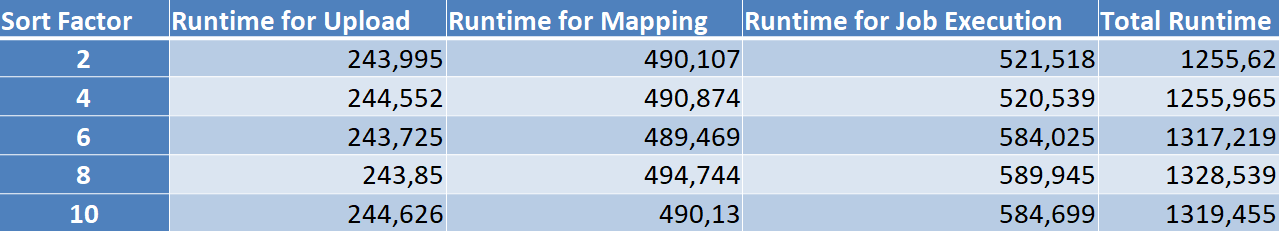
\includegraphics[width=1.0\linewidth]{sortfactor-table.PNG}
	\caption[Caption for LOF]{Sortfactor/RunTime table}
	\label{sortfactor-table}
\end{figure}
The graph in the figure \ref{sort-factor-chart} shows the dependency between the sort factor and the run time:
\begin{figure}[H]
	\centering
	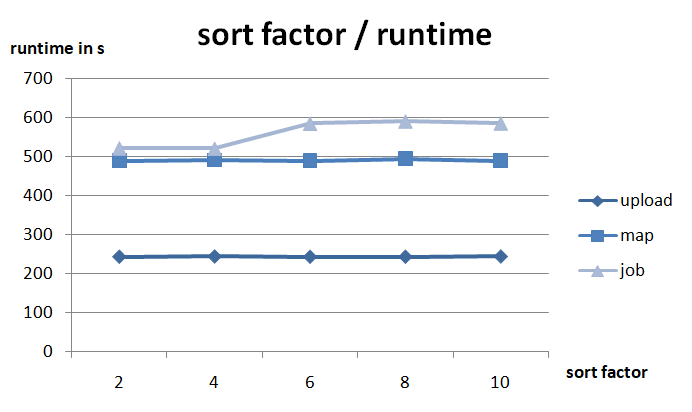
\includegraphics[width=0.75\linewidth]{sort-factor-chart.PNG}
	\caption[Caption for LOF]{Sortfactor/RunTime chart}
	\label{sort-factor-chart}
\end{figure}
Since the sort factor specifies how many parallel streams are used by the simulated cluster to sort the data, it is clear that starting from a certain amount of streams, the performance suffers from this. Figure shows that from a sort factor of 6, the time for shuffling and reducing increases because of this, while the time for the upload and mapping processes stays static.
\section{Changing the requiredMappers and requiredReducers}
The last two parameters to be examined are the \textit{requiredMappers} and \textit{requiredReducers}. The table in figure \ref{mapper-reducer-table} shows the individual value pairs for these two parameters as well as the resulting run times for the simulation.
\begin{figure}[H]
	\centering
	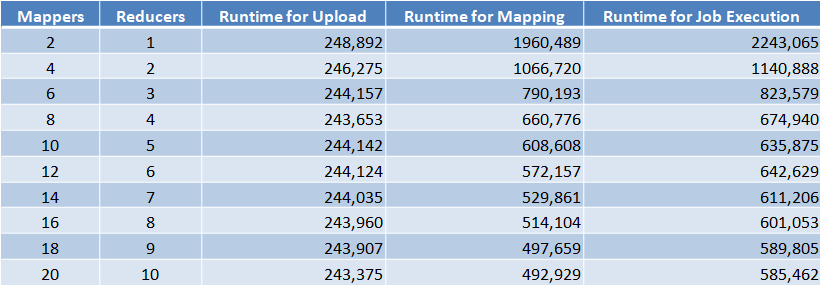
\includegraphics[width=1.0\linewidth]{mapper-reducer-table.PNG}
	\caption[Caption for LOF]{Number of Mappers and number of Reducers/RunTime table}
	\label{mapper-reducer-table}
\end{figure}
The graph in the figure \ref{mappers-reducers-chart} shows the dependency between the amount of mappers and reducers to the run time:
\begin{figure}[H]
	\centering
	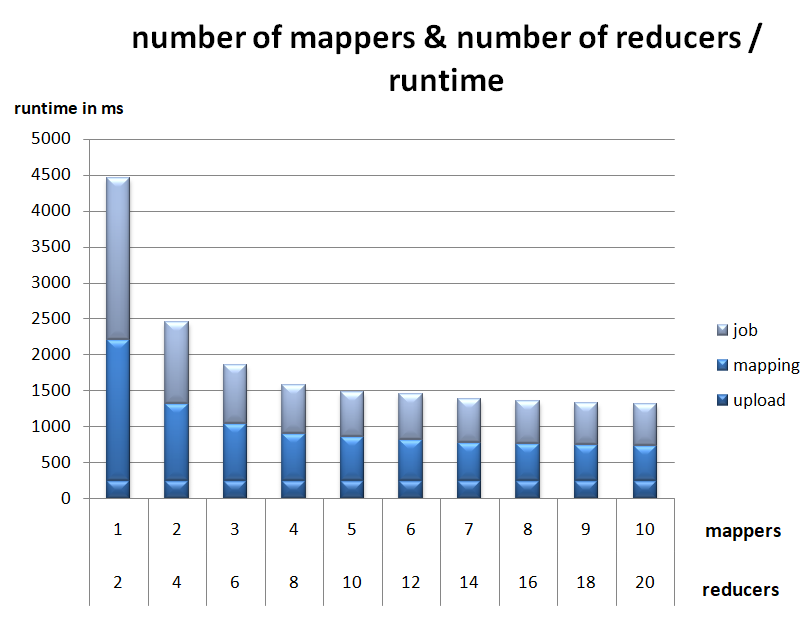
\includegraphics[width=1.0\linewidth]{mappers-reducers-chart.PNG}
	\caption[Caption for LOF]{Number of Mappers and number of Reducers/RunTime chart}
	\label{mappers-reducers-chart}
\end{figure}
As was to be expected, the time required for mapping and reducing decreases exponentially with the increasing number of mappers and reducers processing the data blocks in parallel. With a value of 7 reducers and 14 mappers, the time required is balanced and runs statically with a further increase in the number of mappers and reducers. This is because each MapReduce task involves a certain overhead and requires resources and time for communication and data traffic between mappers and reducers. Therefore, from a certain stage on, there is no point in increasing the number of mappers and reducers. It can even turn out to be a disadvantage, since too many parallel running mappers and reducers have an impact on performance. The time required for the data upload however stays static.
%%%%%%%%%%%%%%%%%%%%%%%%%%%%%%%%%%%%%%%%%%%%%%%%%%%%%%%%%%%%%%%%%%%%%%%%%%%%%%%%%%%%%%%%%%%%%%%%%%%%%%%%%
%%%%%%%%%%%%%%%%%%%%%%%%%%%%%%%%%%%%%%%%%%%%%%%%%%%%%%%%%%%%%%%%%%%%%%%%%%%%%%%%%%%%%%%%%%%%%%%%%%%%%%%%%
%%%%%%%%%%%%%%%%%%%%%%%%%%%%%%%%%%%%%%%%%%%%%%%%%%%%%%%%%%%%%%%%%%%%%%%%%%%%%%%%%%%%%%%%%%%%%%%%%%%%%%%%%
\chapter{Conclusion}
\label{conlusion}
The aim of this workshop was to develop a basic understanding of the programming model \textbf{MapReduce} and its Java implementation \textbf{Hadoop}. Changing individual parameters in the Hadoop simulation \textbf{HSim} showed interesting insights into the runtime behavior of the MapReduce algorithm and strengthens theoretical knowledge by observing a simulated Hadoop environment.
\\
All in all, it can be said that MapReduce is a very powerful technology to process large amounts of data quickly and efficiently. This is particularly true in today's times where the data volumes created by worldwide Internet use are constantly increasing, while at the same time the computing power of individual systems is no longer increasing so quickly and these are therefore overwhelmed by such data volumes.
\\
However, the user must also know what he is doing when configuring Hadoop, as certain changes to the parameters can also affect the performance negatively. This was demonstrated by the changes to the parameters in the evaluation.

